%
%%%%%%%%%%%%%%%%%%%%%%%%%%%%%%%%%%%%%%%%%%%%%%%%%%%%%%%%%%%%%%%%%%%%%%%%%%%%%%%%
\chapter{Theoretical background}\label{chap:1}
%%%%%%%%%%%%%%%%%%%%%%%%%%%%%%%%%%%%%%%%%%%%%%%%%%%%%%%%%%%%%%%%%%%%%%%%%%%%%%%%
%
%%%%%%%%%%%%%%%%%%%%%%%%%%%%%%%%%%%%%%%%%%%%%%%%%%%%%%%%%%%%%%%%%%%%%%%%%%%%%%%%
\section{Introduction}\label{sec:intro}
%%%%%%%%%%%%%%%%%%%%%%%%%%%%%%%%%%%%%%%%%%%%%%%%%%%%%%%%%%%%%%%%%%%%%%%%%%%%%%%%
%
Since the theoretical prediction of skyrmions in \todo{year?}
\todo{cite} and their experimental discovery in \todo{year} \todo{cite},
skyrmions have been extensively investigated both by theorists and
experimentalists \todo{some refs}. Skyrmions have caused a lot of excitement
mostly due to their promising properties that might qualify them as fast and
efficient memory. Three-dimensional non-perturbative classical Monte Carlo
methods developed recently~\cite{skyrmionlattice}, allow us to compute the full
finite temperature phase diagram and explore phase transitions. The goal of this
project was to implement a simulated annealing Monte Carlo code with the
discretized lattice Hamiltonian introduced in~\cite{skyrmionlattice} and
basically reproduce the results discussed there.  In contrast to most work on
Monte Carlo methods for spin lattices with emerging skyrmions, we want to
provide a detailed exposition of the algorithms and numerical aspects. The
report can serve as an ab initio step-by-step introduction on how to write Monte
Carlo methods and discusses associated pitfalls or caveats based on a concrete
example.  All code is publicly available on GitHub under \todo{link} and we hope
that it will be useful to others.

We introduce the model Hamiltonian in \secref{sec:model}. In
\secref{sec:mctheory} we derive Monte Carlo integration and optimization in the
framework of simulated annealing and state some important properties and results
mostly without proofs. Moreover, we discuss practical verification strategies
for Monte Carlo codes. \Secref{sec:code} contains the documentation of Sky-MoCa
as well as a quick start user manual. Finally we also provide reasoning for
design decisions. Some results and analysis of the simulations are presented in
\secref{sec:results}. However, the main goal of this paper is to illuminate the
methods more than to interpret physical results. Finally, we conclude in
\chapref{chap:3}.
%
%%%%%%%%%%%%%%%%%%%%%%%%%%%%%%%%%%%%%%%%%%%%%%%%%%%%%%%%%%%%%%%%%%%%%%%%%%%%%%%%
\section{The Spin Lattice Model}\label{sec:model}
%%%%%%%%%%%%%%%%%%%%%%%%%%%%%%%%%%%%%%%%%%%%%%%%%%%%%%%%%%%%%%%%%%%%%%%%%%%%%%%%
%
A common high-level way to think about magnetism in condensed matter is in terms
of complex collective behavior of spins, each of which is associated with a
magnetic moment. Astoundingly, this figurative model is quite powerful and
allows for a thorough explanation of a wide range of phenomena. Let us consider
a three-dimensional lattice with equidistant spacing in each direction. To each
lattice site we attach a spin, represented by an element of the unit
sphere~$S^2$, see \figref{fig:s2}. In the following we will often resort to the
two-dimensional model for illustration purposes, because it is easier to draw on
a two-dimensional surface as illustrated in \figref{fig:lattice}. However, all
computations solely concern the three-dimensional model. Each vertex of the
lattice could for example represent a nucleus in a solid with a rigid crystal
like structure. Hence the whole lattice can be interpreted as a regular atomic
structure of a solid.

\begin{figure}
  \centering
  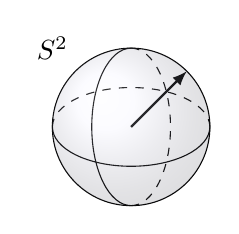
\begin{tikzpicture}
    \draw[->, thick, \select, >=latex] (0,0) -- (45:1cm);
    \draw (-1,0) arc (180:360:1cm and 0.5cm);
    \draw[dashed] (-1,0) arc (180:0:1cm and 0.5cm);
    \draw (0,1) arc (90:270:0.5cm and 1cm);
    \draw[dashed] (0,1) arc (90:-90:0.5cm and 1cm);
    \draw (0,0) circle (1cm);
    \shade[ball color=blue!10!white,opacity=0.20] (0,0) circle (1cm);
    \node at (-1,1) {$S^2$};
  \end{tikzpicture}%
  \caption{We consider three-dimensional spins, \ie{} elements of the unit
  sphere~$S^2$.}
\label{fig:s2}
\end{figure}

\begin{figure}
  \centering
  \begin{tikzpicture}
    \latticeinter{4}
    \begin{scope}[xshift=8cm,yshift=1cm]
      \lattice{4}
    \end{scope}
  \end{tikzpicture}%
  \caption{On the left side we show a two-dimensional spin lattice. Each lattice
  site carries a magnetic moment or spin, represented by an arrow of unit
  length, \ie{}, in the two-dimensional picture, by an element of~$S^1$. The
  neighbors of a lattice site are the ones above, below, left and right in the
  two-dimensional case. The blue squares are the neighbors of the red circle.
  The three-dimensional picture on the right side becomes unclear in a
  two-dimensional drawing rather quickly. Note that the magnetic moments are now
  also three-dimensional, \ie{} elements of the two-dimensional unit
  sphere~$S^2$. In three dimensions each vertex has up to six neighbors.}
\label{fig:lattice}
\end{figure}

\todo{next to 2d and 3d lattice make drawing of only one vertex plus 6 neighbors
in 3 dimensions}

We work with a cubic lattice
%
\begin{equation}
  \Sigma := \numlist{1}{N_x} \times \numlist{1}{N_y} \times
  \numlist{1}{N_z} \subset \bN^3 \subset \bR^3\:,
\end{equation}
%
where we interpret~$(i,j,k) \in \Sigma$ as~$i \hx + j \hy + k \hz
\in \bR^3$. Here,~$\hx, \hy, \hz$ are the standard basis vectors of~$\bR^3$.
Note that we can translate the whole lattice by arbitrary integer linear
combinations of the standard basis vectors, thus starting at~$(1,1,1)$ does not
have any physical meaning. It merely corresponds nicely to the numerical
implementation in any~$1$-indexed programming language. At each point~$\r \in
\Sigma$ we attach a spin~$\S_{\r} \in S^2$, which yields the overall
configuration space~$\Pi := \prod_{\r \in \Sigma} S^2$.  Each element of~$\Pi$
consists of~$\abs{\Sigma}=N_x N_y N_z$ spins, \ie{} elements of~$S^2$, thus
describes one possible spin configuration of the whole lattice. We refer to the
specific spin at position~$\r \in \Sigma$ with~$\S_{\r} \in S^2$.  Note that
only the positions of the spins are discretized, but not explicitly their
directions. In any real implementation there is always a fine grained
discretization caused by the finite number of representable of floating point
numbers. Discrete vertices and continuous spins mirror nicely the natural
crystal structure of solids.

In a typical physical simulation one might want to find the ground state of this
system, \ie{} the lowest energy state, for some given external and internal
parameters. Necessarily, we need to define some notion of energy and also
identify some possible parameters for the spin lattice. Apparently any physical
measure of energy must be based on interactions between the spins within the
system or with external fields. Let us elaborate on some possible interactions.
Each of them comes with a constant that can be interpreted as a weight, \ie{}
how much the respective interaction contributes to the energy with respect to
the others. Let us already take away that those constants are potential
parameters of the system.

\subsection{Interactions}

\subsubsection{Ferromagnetic/direct exchange}

The most obvious interaction is the \newterm{ferromagnetic} or \newterm{direct}
exchange.  Pictorially speaking, it favors constellations where spins that are
close to each other point into the same direction. A system only interacting
this way will end up in a state where all spins are parallel to each other. The
measure for parallelism of two neighboring spins~$\S_{\r_1}, \S_{\r_2} \in S^2$
can be expressed as
%
\begin{equation}
  -\S_{\r_1} \cdot \S_{\r_2} =
  -\norm{\S_{\r_1}} \norm{\S_{\r_2}} \cos(\alpha) \:,
\end{equation}
%
where~$\alpha$ is the angle between~$\S_{\r_1}$ and~$\S_{\r_2}$. The minus sign
ensures that the energy of two parallel spins is actually smaller than the
energy of two perpendicular or even antiparallel ones.  In the continuum theory
of magnetic moments, the direct exchange term consists of a gradient, which is a
local quantity, \ie{} the gradient at a point only depends on an arbitrarily
small neighborhood of the point. Thus we will always consider the ferromagnetic
exchange to be \newterm{local} or \newterm{short ranged} in the sense that it
only contributes for adjacent lattice sites, as shown in \figref{fig:lattice}.

\subsubsection{Interaction with an external field}

Another important exchange term describes the interaction of the system with an
\newterm{external magnetic field}. Clearly, every spin tries to align with an
external field~$\B$, which we express mathematically via~$-\B \cdot \S$ for
every spin~$\S$ on the lattice. This contribution is also called the
\newterm{Zeeman energy}. It can be misleading to use terms such as
\newterm{non-local} or \newterm{long ranged} for this exchange, since it is not
an interaction between two or more spins within the system, but affects each
lattice site independently in the same way. Naturally, for the external
field,~$\B$ itself is the parameter of the interaction.

\subsubsection{Dipole-dipole interaction}

The \newterm{dipole-dipole interaction} is somewhat more complex, but also
weaker.  For two spins~$\S_{\r_1}, \S_{\r_2} \in S^2$, it is given by
%
\begin{equation}
  - {\norm{\r}^{-3}} (3 (\S_{\r_1} \cdot \hat{\r})
  (\S_{\r_2} \cdot \hat{\r}) - \S_{\r_1} \cdot \S_{\r_2})\:,
\end{equation}
%
where~$\r = \r_2 - \r_1$ and~$\hat{\r} = \r / \norm{\r}$ points from the
location of the first spin to the location of the second one. The dipole-dipole
interaction depends on the distance between the two lattice sites as well as the
orientation of the two spins not only relative to each other, but also to the
line connecting them. Moreover, the explicit dependence on the relative position
already indicates that the dipole-dipole interaction is relevant for each pair
of magnetic moments in the system, it is a long ranged interaction. In an~$N^3$
lattice, the number of pairs scales like~$N^6$. As a consequence, most
simulations do not take the dipole-dipole exchange into account purely due to
limited computational resources. We will also disregard the dipole-dipole
exchange.

\subsubsection{Dzyaloshinskii-Moriya exchange}

In this work we are interested in certain crystals that lack inversion symmetry,
\eg{} MnSi, and thus exhibit chiral magnets. The missing inversion symmetry
gives rise to the so called \newterm{weak Dzyaloshinskii-Moriya} (DM) coupling.
In the continuum it is described by a term proportional to~$-\S(\r) \cdot
(\nabla \times \S(\r))$. Just like the gradient, the curl of a vector field is a
local property, thus the DM exchange only contributes for adjacent lattice
sites. The discretized version for two spins~$\S_{\r_1}, \S_{\r_2} \in S^2$ at
neighboring positions~$\r_1, \r_2 \in \Sigma$ reads
\begin{equation}
  - (\S_{\r_1} \times \S_{\r_2}) \cdot (\r_2 - \r_1)\:.
\end{equation}
%
Since the cross product is zero for parallel vectors and maximal for
perpendicular ones, the DM coupling acts against the ferromagnetic interaction
and favors constellations where adjacent spins are perpendicular to each other.

\subsection{The Hamiltonian}

\subsubsection{Summing up the interactions}

Let us now combine the FM and DM interaction as well as an external magnetic
field to compute the energy for the lattice~$\Sigma$. To this end we add up the
contributions from each spin and for each interaction. For instance, the
external field exchange term simply becomes
%
\begin{equation}\label{Bsum}
  -\sum_{\r \in \Sigma} \S_{\r} \cdot \B\:.
\end{equation}
%

Adding up the terms for the FM interaction with all direct neighbors naively as
in
%
\begin{equation}\label{FMsumnaive}
  -\sum_{\r \in \Sigma} \S_{\r} \cdot (\S_{\r + \hx} + \S_{\r - \hx} +
    \S_{\r + \hy} + \S_{\r - \hx} + \S_{\r + \hz} + \S_{\r - \hz})\:,
\end{equation}
%
poses two problems. First, apparently in this fashion we count the interaction
between some pairs of spins multiple times. If~$\Sigma$ was an infinite grid,
\ie{}~$\Sigma=\bZ^3$, we would count every pair exactly twice and could simply
divide~\eqref{FMsumnaive} by two. However,~$\Sigma$ is finite which leads
to the second more subtle issue. Not every lattice site has a neighbor in each
direction~$\hx, \hy, \hz$. Consider the spin in the lower right corner of a
lattice in \figref{fig:lattice}. The sum in our first naive expression for the
FM interaction~\eqref{FMsumnaive} suggests that we need its right and lower
neighbor, which apparently do not exist. As a consequence, we need to define
some behavior at the boundaries. There are several ways to do this and a
plausible treatment of boundary conditions is a central aspect of many different
areas in scientific computing. It is important to realize that this is not
simply an implementation nuisance that we can get rid off by any means that make
the code work. Various boundary conditions represent different physical systems
and can significantly alter the results of a simulation.

\subsubsection{Boundary conditions}

In many cases the desired simulation volume is an infinite space, or at least so
large compared to all internal length scales that it is practically infinite. On
physical computing machines we are always limited to finite spaces. The most
obvious way for finite systems is to set all spins outside of~$\Sigma$ to zero,
\ie{}~$\S_\r = 0$ for all~$\r \in \bZ^3 \setminus \Sigma$. Consequently the
lattice sites on the boundary have less neighbors to interact with. This is
called an \newterm{open boundary}. Open boundaries are often undesirable,
because they heavily impact the behavior. In our example, a magnetic moment at
the boundary is less effected by the FM and DM interaction, simply because it
has less neighbors. However, the external field still has the same impact on a
boundary spin. This imbalance leads to polarized spins at the boundaries, \ie{}
they tend to point right in the direction of the external magnetic field~$\B$ to
maximize their Zeeman energy.

One common way to get out of this dilemma is to implement \newterm{periodic
boundary conditions}. We think of our lattice as a finite box of volume~$L^3$
for~$L\in \bRp$ and simply replicate that box infinitely many times to fill the
whole space, see \figref{fig:periodic} for a two-dimensional illustration. In
practice, we will access the lattice sites by indexing a three-dimensional array
with indices~$(i,j,k)\in\Sigma$. Whenever the algorithm tries to index out of
bounds, \eg{} requests~$j=N_y + 1$, we simply use~$j=1$ again. For~$i=0$ we
use~$i=N_x$,~$k=N_z+2$ is replaced by~$k=2$ and so on. In general, this behavior
can be achieved by always working with the indices
%
\begin{equation}\label{periodicindices}
  ((i-1 \mod N_x) + 1, (j-1 \mod N_y) + 1, (k-1 \mod N_z) + 1) \in \Sigma
\end{equation}
%
whenever the algorithm requests data at position~$(i,j,k) \in \bZ^3$. By
construction, those new indices always lie in~$\Sigma$. We can now
unproblematically include spins at officially non-existing positions in our
mathematical expressions, implicitly assuming that those are being wrapped
around periodically to positions within the lattice. This way every vertex has
the same number of neighbors.

\begin{figure}
  \centering
  \begin{tikzpicture}
    \periodic{}
  \end{tikzpicture}
  \caption{We illustrate periodic boundary conditions for a
  two-dimensional~$4\times4$ grid. The actually implemented simulation value is
  given by the shaded square in the middle. This square is copied over and over
  again in all directions as indicated by the surrounding lattice sites. Note
  how the four boundaries of the square keep their orientation throughout that
  copying procedure. While it appears like we have filled an infinite space, all
  red squares are identified, because they are represented internally by only
  one vertex in the central square. The same holds true for the green
  pentagons of course. If our code needs the value of the right neighbor of the
  green pentagon in the central square for example, we can instead pick the
  right neighbor of \emph{any} green pentagon. One of those will always lie in
  the center square again and thus be available in memory.}
\label{fig:periodic}
\end{figure}

In our first simulations, we will employ periodic boundary conditions in all
three directions using~\eqref{periodicindices}. For other scenarios we opened up
the boundaries in one direction. This solves the second issue we encountered
in~\eqref{FMsumnaive}.

\subsubsection{Combining all interactions}

Now that we have established a well defined behavior at the boundary, we can
also tackle the first problem of counting interactions multiple times. For
periodic boundary conditions we could divide the whole expression by~$2$. In the
implementation we do not want to actually carry out redundant computations, thus
we work with
%
\begin{equation}\label{FMsum}
  -\sum_{\r \in \Sigma} \S_{\r} \cdot
    (\S_{\r + \hx} + \S_{\r + \hy} + \S_{\r + \hz})\:.
\end{equation}
%
It is worth convincing oneself that in this expression with periodic boundary
conditions every pair of neighboring lattice sites is included exactly once and
it also yields the correct results for open boundaries.

Finally, the DM term for the whole lattice is
%
\begin{equation}\label{DMsum}
  -\sum_{\r \in \Sigma} ((\S_{\r} \times \S_{\r + \hx}) \cdot \hx +
    (\S_{\r} \times \S_{\r + \hy}) \cdot \hy +
    (\S_{\r} \times \S_{\r + \hz}) \cdot \hz)\:.
\end{equation}
%
Everything we discussed about boundary conditions for the FM exchange also holds
true for the DM interaction.

Ultimately adding up all interactions~\eqref{Bsum},~\eqref{FMsum}
and~\eqref{DMsum}, we obtain the Hamiltonian, \ie{} the energy of the system in
a given configuration~$\pi \in \Pi$
%
\begin{align}\label{hamiltonian}
  H(\pi) = &-\sum_{\r \in \Sigma}\biggl(\S_{\r} \cdot \B +
      J \S_{\r} \cdot (\S_{\r+\hx} + \S_{\r+\hy} + \S_{\r+\hz}) \\
      &+ K (\S_{\r} \times \S_{\r+\hx} \cdot \hx +
            \S_{\r} \times \S_{\r+\hy} \cdot \hy +
            \S_{\r} \times \S_{\r+\hz} \cdot \hz)\biggr)\:.
\end{align}
%
The parameters~$J$,~$K$ and~$\B$ are sometimes used synonymously for the
ferromagnetic, the Dzyaloshinskii-Moriya and the external field interaction
terms. As we will see in the simulation results in \chapref{chap:3}, the
physical behavior of the system strongly depends on these freely adjustable
parameters. For a given set of parameters and at zero temperature we typically
define the physical configuration to be the
%
\begin{equation}\label{objective}
  \argmin_{\pi \in \Pi} H(\pi)\:.
\end{equation}
%

\subsubsection{Anisotropies}

% While we have remedied the problem of unwanted boundary effects due to missing
% neighbors, we are still working in a finite volume. While any real crystal also
% has a finite volume, it can typically be considered infinite relative to the
% lattice spacing. Due to computational limitations we can only simulate lattices
% with roughly~$30^3$ vertices. Thus the whole lattice is only~$30$ orders of
% magnitudes longer than the lattice spacing which leads to significant
% \newterm{finite size effects}.

In~\eqref{hamiltonian} we have collected all interactions on the lattice. Those
stem from a continuum model. Therefore we have to expect discretization errors.
In particular, the transition to a finite cubical lattice introduces
anisotropies that are absent in the original continuum model. Buhrandt and Fritz
show in~\cite{skyrmionlattice} that we can partly compensate for those
disruptive anisotropies by adding next-nearest neighbor interactions to the
Hamiltonian. The optimal choice to render higher order deviations from the
continuum model as small as possible is
%
\begin{align}\label{hamiltonianfull}
  H' := & \sum_{\r \in \Sigma} \biggl(
  \frac{J}{16} \S_{\r} \cdot (\S_{\r+2\hx} + \S_{\r+2\hy} + \S_{\r+2\hz}) \\
  &+ \frac{K}{8} (\S_{\r} \times \S_{\r+2\hx} \cdot \hx +
        \S_{\r} \times \S_{\r+2\hy} \cdot \hy +
        \S_{\r} \times \S_{\r+2\hz} \cdot \hz)\biggr)\:.
\end{align}
%
The Hamiltonian used in the simulation is then~$H + H'$. Note that~$H'$ has the
same structure of the FM and DM term of~$H$, but enters with smaller constant
and opposite sign. Adding next-nearest neighbor interactions computationally
makes a difference, but is handled the exact same way as nearest neighbor
interactions, see \figref{fig:interact}. Periodic and open boundaries still work
exactly the same way.

\begin{figure}
  \centering
  \begin{tikzpicture}
    \latticeselect{5}
    \begin{scope}[xshift=5cm]
      \latticeinter{5}
    \end{scope}
    \begin{scope}[xshift=10cm]
      \latticeinternn{5}
    \end{scope}
  \end{tikzpicture}%
  \caption{We select a spin at position~$\r \in \Sigma$ (left), show the nearest
  neighbors (middle) and the next-nearest neighbors (right). Note that although
  the diagonally neighboring vertices are closer to~$\r$ than the next-nearest
  neighbors, they are not included in any interaction.}
\label{fig:interact}
\end{figure}

\subsection{A note on parameter values}

Recall that there is a great conflict of interest between the FM and
the DM interactions. While the FM term in the Hamiltonian is minimal when all
spins are parallel to each other, the DM term favors a configuration where
neighboring spins are orthogonal. The specific compromise between those effects
depends mostly on their respective strength~$J$ and~$K$. In reality the direct
interaction~$J$ is much stronger and one typically encounters helical
structures with long modulation periods, see \todo{figref}. \todo{If J is
typically larger, why is here J smaller?} For example in MnSi the spins wind
around a given modulation axis only once per roughly~$40$ lattice spacings. By
tuning the ratio~$J/K$ we can set the periodicity. For a period of~$N$ lattice
sites, we have to set~$J/K$ to~$\tan(2\pi / N)$. In all our simulations we
chose~$J=1$ and~$K=\tan(2\pi / 10)$. Moreover, we let the external magnetic
field point in the~$\hz$ direction~$\B=(0,0,B)$.

We can fix one of the parameters, in this case~$J$, arbitrarily and then work in
abstract lattice units. A computer can only deal with dimensionless numbers and
in numerical simulations one often makes some convenient, but arbitrary choices.
It is then sometimes quite difficult to translate the results to physically
meaningful values.

The alert reader might have realized that so far our model does not contain any
thermal energy. When talking about magnetism, temperature typically has a strong
influence on the physical properties of various materials. However,
incorporating a temperature dependent term into the Hamiltonian that accounts
for the thermal energy is quite a challenge.  Any additive term that depends
solely on the temperature will not have any effect on~\eqref{objective}. On the
other hand there is no physical reason for complex interaction terms that
actually yield different configurations for different temperatures. Our
intuition tells us that thermal energy is intrinsically of dynamic nature, thus
cannot be captured in a single static spin configuration. In fact we will
account for temperature in the optimization algorithm itself and clearly see the
dynamic nature of it in \secref{sec:mctheory}.

\subsection{Summary}

In this section we have set up our model, which we will briefly summarize. We
work on the lattice
%
\begin{equation}
  \Sigma := \numlist{1}{N_x} \times \numlist{1}{N_y} \times
  \numlist{1}{N_z} \subset \bN^3 \subset \bR^3\:
\end{equation}
%
and attach a spin~$\S_{\r} \in S^2$ to each lattice site~$\r \in \Sigma$. This
yields the configuration space
%
\begin{equation}
  \Pi := \prod_{\r \in \Sigma} S^2\:.
\end{equation}
%
On~$\Pi$ we define the Hamiltonian~\eqref{hamiltonianfull} where we implement
periodic (and sometimes partially open) boundary conditions. We fix the
parameters~$J=1$ and~$K=\tan(2\pi / 10)$ of the FM and DM interaction, which
leaves us only with the magnetic field in the~$\hz$ direction~$B$. In the next
section we will introduce the temperature as a second parameter. Very roughly
speaking, for given values of~$B$ and~$T$ we then seek to minimize~$H(\pi)$. The
minimizing configuration is considered to be the physical one.
%
%%%%%%%%%%%%%%%%%%%%%%%%%%%%%%%%%%%%%%%%%%%%%%%%%%%%%%%%%%%%%%%%%%%%%%%%%%%%%%%%
\section{General Monte Carlo methods}\label{sec:mctheory}
%%%%%%%%%%%%%%%%%%%%%%%%%%%%%%%%%%%%%%%%%%%%%%%%%%%%%%%%%%%%%%%%%%%%%%%%%%%%%%%%
%
Now that we have clearly stated the model, let us dive into the numerics. Monte
Carlo methods stand for a broad class of numerical algorithms that are based on
some sort of repeated random sampling. The term actually stems from the casinos
in Monte Carlo, where gamblers bet on the outcome of random processes. It is
hard to formulate a more specific feature that all Monte Carlo algorithms have
in common. Most often, Monte Carlo techniques are used for optimization,
integration or sampling probability distributions. We will see soon, that
besides optimization our problem will also require us to perform
high-dimensional integrals. Before we describe our algorithm of choice in
detail, we have to issue a warning. While Monte Carlo methods are generally easy
to implement and can be applied blindly to virtually any problem, they are
almost always hopelessly inferior to specialized techniques in terms of accuracy
and efficiency. They should be the last resort after everything else has failed.
Let us start out with a general description of Monte Carlo integration and
optimization.

\subsection{Integration}

\subsubsection{Overview and comparison of integration methods}

The most naive numerical integration methods make use of interpolating
functions. They sample the integrand at a fixed finite number of base points in
the domain and approximate the integrand by an interpolation that is easy to
integrate. Consider for example the trapezoidal rule. It samples the integrand
on a homogeneous grid and approximates it by a piecewise linear function between
the grid vertices, see \figref{fig:int}. The integral of a piecewise linear
function is easily computed by adding up the areas of the trapezoids underneath
the curve. The larger the number of base points, \ie{} the smaller the grid
spacing, the more accurate the result for sufficiently well behaved integrands.
The important aspect here is that for a given integration rule and a given
number of base points the choice of nodal points in the domain is completely
deterministic. More sophisticated routines choose refine the grid of base points
iteratively in regions, where the error is above a certain accuracy and
precision goal. But even such \newterm{adaptive} methods have fixed rules how
the new samples have to be chosen. Typically that determinism brings great
advantage, because one can prove optimality results and certain error bounds for
the choice of base points.

In contrast, Monte Carlo techniques draw the samples randomly from some
probability distribution. The general idea is illustrated by the following
example. From the definition of the expectation value we have
%
\begin{equation}\label{mcsimple}
  \int_a^b f(x) \sucd{x} = (b-a) E_{\cU_{[a,b]}}(f)\:,
\end{equation}
%
where~$E_{\cU_{[a,b]}}$ is simply the expectation value over the uniform
distribution~$\cU$ on the interval~$[a,b]$. The expectation value can be
approximated by averaging~$f$ over~$N \in \bN$ independent samples~${x_i}$
of~$\cU_{[a,b]}$
%
\begin{equation}\label{evapprox}
  E_{\cU_{[a,b]}}(f) \approx \frac{1}{N} \sum_{i=1}^N f(x_i)
\end{equation}
%
and thus
%
\begin{equation}\label{mcsapprox}
  \int_a^b f(x) \sucd{x} \approx \frac{b-a}{N} \sum_{i=1}^N f(x_i)\:.
\end{equation}

Both paradigms, the trapezoidal rule as well as the Monte Carlo sampling, are
illustrated for a simple one-dimensional function in the top row
of~\figref{fig:int}. In this one-dimensional scenario the Monte Carlo
integration is absolutely not competitive. Even the crude trapezoidal rule will
easily outperform it in terms of accuracy, precision and also efficiency for any
given number of base points~$N$. It turns out that the error of the trapezoidal
rule scales like~$1/N^2$. Piecewise quadratic approximation, called Simpon's
rule or Kepler rule, already brings the error down to~$1/N^4$. Hence these
methods converge extremely fast for suitable integrands. Keep in mind we are
talking about the simplest rules imaginable which are hardly ever used in
practice. State of the art integration methods are by far more sophisticated
with still better convergence properties for a certain classes of functions.
However, to exploit the full potential of specialized integration routines one
still has to have some idea of what the integrand looks like. Periodic functions
call for other routines than slightly singular functions with strongly localized
features for instance.  Furthermore even adaptive rules require to at least
crudely sample the whole integration domain. In a ten-dimensional integral, even
a coarse grid of ten base points in each direction requires~$10^{10}$ function
evaluations. Let us contrast these insights with the errors in Monte Carlo
integration.

\subsubsection{Error of Monte Carlo integration}

First of all, the law of large numbers ensures that the
approximation~\eqref{evapprox} converges for large~$N$
%
\begin{equation}
  \lim_{N \to \infty} \frac{1}{N} \sum_{i = 1}^N f(x_i) = E_{\cU_{[a,b]}}(f)\:.
\end{equation}
%
Let us henceforth use~$I$ and~$\hat{I}$ for the exact and approximate values of
the integral
%
\begin{equation}
  I := \int_a^b f(x) \sucd{x} \qqtxtqq{and}
  \hat{I} := \frac{b-a}{N} \sum_{i=1}^N f(x_i)\:.
\end{equation}
%
As usual the variance of~$f$ is given by
%
\begin{equation}
  \sigma^2(f) = \int_a^b (f(x) - I)^2 \sucd{x}\:.
\end{equation}
%
To measure the error in~$\hat{I}$ we consider the~$x_i$ independently
identically distributed random variables with distribution~$\cU_{[a,b]}$. One
can then show that the squared error of the Monte Carlo approximation is
%
\begin{equation}\label{mcerror}
  E_{x_1, \dots , x_N}\bigl((\hat{I} - I)^2\bigr) =
  \frac{1}{(b-a)^N}\int_a^b \pred{x_1} \cdots \int_a^b \pred{x_N}
  \biggl(\frac{b-a}{N} \sum_{i=1}^N f(x_i) - I\biggr)^2 =
  \frac{\sigma^2(f)}{N}\:.
\end{equation}

What this tells us is that the average error we make in the Monte Carlo
integration is~$\sigma(f)/\sqrt{N}$. It is important to realize that with truly
random numbers, each separate run of the same Monte Carlo integration will
generally yield different results. For any single one of them the error could be
much larger than, but for infinitely many runs the error would average to the
standard deviation of~$f$ divided by~$\sqrt{N}$. In stark contrast,
interpolation methods like the trapezoidal rule actually allow you to determine
a strict upper bound of the error for any function meeting some
differentiability criteria.

The single most important result of Monte Carlo integration is that the factor
of~$\sqrt{N}$ is independent of the dimension of the integration domain. This
tells us that even in a~$10^3$ dimensional integration, where interpolation and
adaptive methods would fail straightaway, we can be sure that the average error
scales like~$1/\sqrt{N}$, where~$N$ is the number of samples. This is the key
justification for the use of Monte Carlo methods. Keep in mind, however, that a
convergence rate of~$1/\sqrt{N}$ is tantalizingly slow compared to what we are
used from other numerical algorithms. For example, consider the integral
%
\begin{equation}
  I := \int_0^1 e^{-x} \sucd{x}\:.
\end{equation}
%
Assume we want the error~$\sigma (e^{-x}) / \sqrt{N}$ to be smaller
than~$5 \cdot 10^{-4}$. We compute
%
\begin{equation}\label{sigmaexp}
  \sigma (e^{-x}) =
    \sqrt{E_{\cU_{[0,1]}}(e^{-2 x}) - E_{\cU_{[0,1]}}(e^{-x})^2} =
    0.18098\ldots \:,
\end{equation}
%
which leads to a minimal~$N$ of roughly~$2\cdot10^5$ to achieve our accuracy
goal. We need a couple hundred thousand function evaluations for a moderate
error in a very simple and well behaved integral. For comparison, the
trapezoidal rule reaches the same accuracy for about~$15$ base points, see
\figref{fig:int}.

\subsubsection{Importance sampling}

While the~$N$ dependence in the error of Monte Carlo integration is certainly
more important, because it is the one we have full control over, it pays off to
also elaborate on the standard deviation of the integrand~$\sigma(f)$. Although
the integrand is usually fixed by the problem, there are some tricks to improve
the error by decreasing the variance of the integrand. Let us start from a
generic integral
%
\begin{equation}
  \int_{\Omega \subset \bR^n} f(x) \sucd{\lambda}^n(x)\:,
\end{equation}
%
where~$\lambda^n$ is the ordinary Lebesgue measure on~$\bR^n$. Next, let us
rewrite this as
%
\begin{equation}
  \int_{\Omega \subset \bR^n} f(x) \sucd{\lambda}^n(x) =
    \int_{\Omega \subset \bR^n} \frac{f(x)}{p(x)} p(x) \sucd{\lambda}^n(x) =
    \int_{\Omega \subset \bR^n} \frac{f(x)}{p(x)} \sucd{\mu}(x) =
    E_{p}\biggl(\frac{f(x)}{p(x)}\biggr) \:,
\end{equation}
%
where~$p$ is the probability density function of some measure~$\mu$ on~$\Omega$.
Since we have changed the integration measure, we can now approximate the
integral by
%
\begin{equation}
  \int_{\Omega \subset \bR^n} f(x) \sucd{\lambda}^n(x) \approx
  \frac{\lambda^3(\Omega)}{N} \sum_{i=1}^N \frac{f(x_i^p)}{p(x_i^p)}\:,
\end{equation}
%
where the~$x_i^p$ are now independent samples from the probability distribution
induced by~$p$. The key point is that the error estimate is unaffected by the
measure and thus reads
%
\begin{equation}
  \frac{\sigma(f/p)}{\sqrt{N}} \:.
\end{equation}
%
While we can not change the standard deviation of~$f$, we can now try to
minimize the variance of the ratio~$f/p$ by choosing~$p$ wisely. An optimal
choice would mean~$f/p = \const$. This shows that~$p$ should be large/small
where~$f$ is large/small, which makes sense intuitively. We concentrate the
samples in regions where the contributions to the integral are large. Regions
where~$f$ is insignificantly small will only be samples sparsely. Therefore we
call the procedure \newterm{importance sampling}.

For this method to work in practice, one needs to be able to efficiently sample
the distribution induced by~$p$. In general this is a difficult task and a lot
of research has gone into generating good pseudo random numbers following
arbitrary probability distributions. Moreover, Monte Carlo integration is
typically used precisely when we do not know much about~$f$, hence cannot
choose~$p$ adequately upfront. There are algorithms based on importance
sampling, for example VEGAS, that update~$p$ in real time during the integration
to concentrate on important regions. However, it turns out that many integrals
that come up in physics, particularly in statistical physics as we will see
later, are of the form
%
\begin{equation}\label{probform}
  \int_{\Omega \subset \bR^n} f(x) p(x) \sucd{\lambda}^n(x)\:,
\end{equation}
%
where~$p$ is a probability density function of some measure~$\mu$ on~$\Omega$.
In this case we can directly rewrite the integral as
%
\begin{equation}
  \int_{\Omega \subset \bR^n} f(x) \sucd{\mu}(x) \approx
  \frac{\lambda^3(\Omega)}{N} \sum_{i=1}^N {f(x_i^p)}\:.
\end{equation}
%
Usually~$\sigma(f)$ is smaller than~$\sigma(f\cdot p)$ and as long as we can
sample~$p$ efficiently, we can improve the error for the same~$N$.

Let us illustrate importance sampling with an example. On the right side of the
second row of \figref{fig:int} we plot the function~$e^{-x}$ and some
uniformly distributed random sample points for ordinary Monte Carlo integration.
The bulk of the area under the curve is on the left, while the long exponential
tail can practically be neglected. However, many of our uniformly chosen samples
fall into the right half, where the function is basically zero. At the same
time we undersample the important region. The rather large variation
of~$e^{-x}$ leads to rather large errors as we have discovered
in~\eqref{sigmaexp}. Fortunately, with the right normalization~$e^{-x}$ is a
probability density function that can be sampled efficiently on a computer. The
integral~$\int_0^1 e^{-x} \sucd{x}$ is of the form~\eqref{probform} with
%
\begin{equation}
  f(x) =\frac{e}{e-1} \qqtxtqq{and} p(x) =\frac{e^{1-x}}{e-1}\:.
\end{equation}
%
In this case the Monte Carlo approximation becomes trivial
%
\begin{equation}
  \frac{1}{N} \sum_{i=1}^N \frac{e}{e-1} = \frac{e}{e-1} \:,
\end{equation}
%
which is the exact value of the integral, see last row of \figref{fig:int}. In
this simplified case the integrand itself was up to normalization a probability
distribution. Hence we already computed the integral exactly by finding the
normalization constant for~$p$. In real use cases the function~$f$ would not be
constant and we would have to collect more than just one sample for a reasonable
estimate.

\begin{figure}
  \centering
  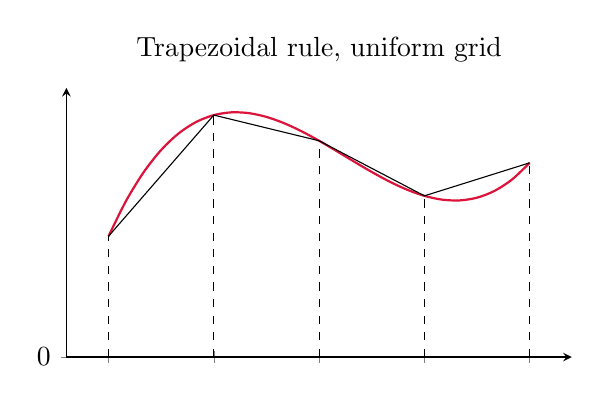
\begin{tikzpicture}[declare function={f=100 - x - 6*x^2 + x^3;}]
    \begin{axis}[
        width=8cm,
        height=5cm,
        ymin=0,
        axis lines=left,
        enlarge y limits=upper,
        enlarge x limits,
        ytick={0},
        xticklabels={,,},
        domain=-2.5:5.5,
        xtick={-2.5, -0.5, ..., 5.5},
        title={Trapezoidal rule, uniform grid},
      ]
      \addplot[thick, Crimson, smooth] {f};
      \addplot[dashed, samples=5, ycomb] {f};
      \addplot[samples=5] {f};
    \end{axis}
  \end{tikzpicture}%
  \hspace{1cm}
  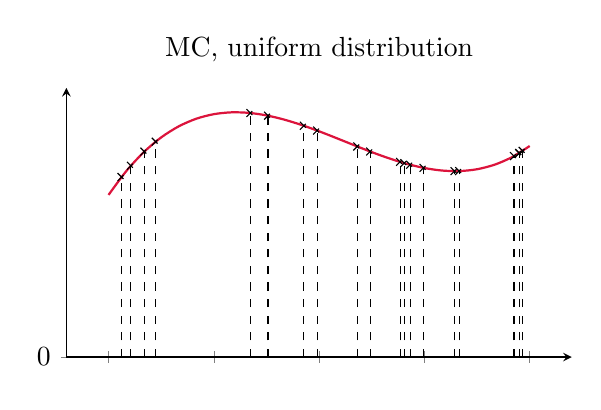
\begin{tikzpicture}[declare function={f=150 - x - 6*x^2 + x^3;}]
    \begin{axis}[
        width=8cm,
        height=5cm,
        ymin=0,
        axis lines=left,
        enlarge y limits=upper,
        enlarge x limits,
        ytick={0},
        xticklabels={,,},
        domain=-2.5:5.5,
        xtick={-2.5, -0.5, ..., 5.5},
        title={MC, uniform distribution},
      ]
      \addplot[thick, Crimson, smooth] {f};
      \addplot[dashed, mark=x, samples at={3.48308, 5.29824, 1.20917,-1.60499,
      3.03779, 1.46106, 3.22893, 4.07112, 2.2248, 4.15928, 5.2014,-2.25321,
      5.30407, 0.19369,-1.81973, 2.46947,-2.07559, 3.11756, 5.36544, 0.529774},
      ycomb] {f};
    \end{axis}
  \end{tikzpicture}%
  \\
  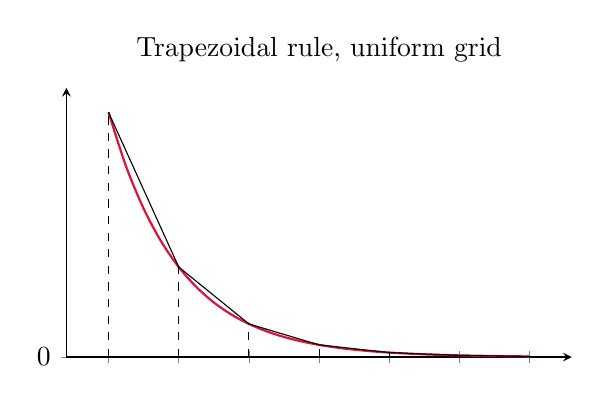
\begin{tikzpicture}[declare function={f=exp(-x);}]
    \begin{axis}[
        width=8cm,
        height=5cm,
        ymin=0,
        axis lines=left,
        enlarge y limits=upper,
        enlarge x limits,
        ytick={0},
        xticklabels={,,},
        domain=0:6,
        xtick={0,...,6},
        title={Trapezoidal rule, uniform grid},
      ]
      \addplot[thick, Crimson, smooth] {f};
      \addplot[dashed, samples=7, ycomb] {f};
      \addplot[samples=7] {f};
    \end{axis}
  \end{tikzpicture}%
  \hspace{1cm}
  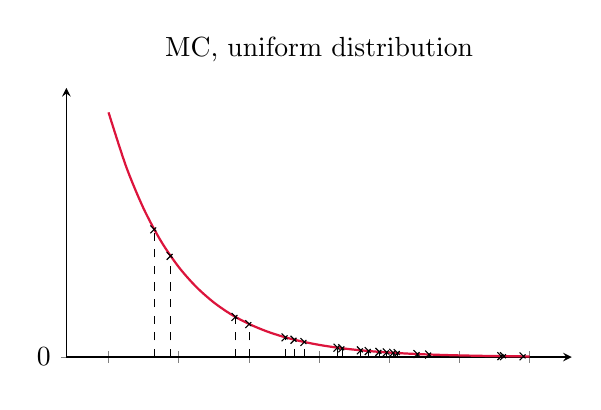
\begin{tikzpicture}[declare function={f=exp(-x);}]
    \begin{axis}[
        width=8cm,
        height=5cm,
        ymin=0,
        axis lines=left,
        enlarge y limits=upper,
        enlarge x limits,
        ytick={0},
        xticklabels={,,},
        domain=0:6,
        xtick={0,...,6},
        title={MC, uniform distribution},
      ]
      \addplot[thick, Crimson, smooth] {f};
      \addplot[dashed, mark=x, samples at={2.79019, 3.26148, 0.650803, 5.91188,
      5.63303, 2.00519, 3.33023, 4.05605, 4.11961, 5.59612, 3.85836, 0.883656,
      3.70697, 2.64962, 1.80842, 2.52199, 4.56677, 3.59437, 4.40159, 3.96445},
      ycomb] {f};
    \end{axis}
  \end{tikzpicture}%
  \\
  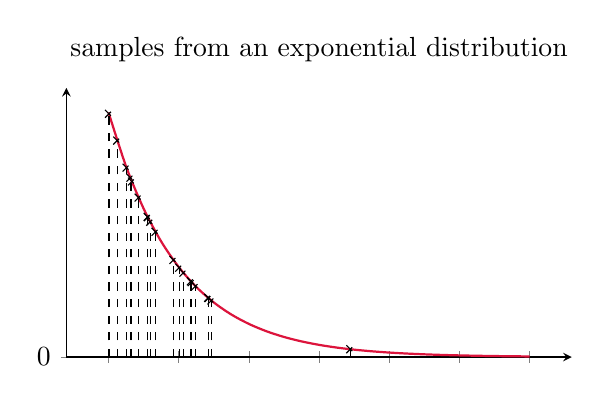
\begin{tikzpicture}[declare function={f=exp(-x);}]
    \begin{axis}[
        width=8cm,
        height=5cm,
        ymin=0,
        axis lines=left,
        enlarge y limits=upper,
        enlarge x limits,
        ytick={0},
        xticklabels={,,},
        domain=0:6,
        xtick={0,...,6},
        title={samples from an exponential distribution},
      ]
      \addplot[thick, Crimson, smooth] {f};
      \addplot[dashed, mark=x, samples at={1.17301, 0.559973, 0.256368, 1.00665,
      1.23844, 0.00605024, 3.44436, 0.122949, 0.311557, 0.428481, 1.06569,
      1.4651, 0.669611, 1.18508, 1.41826, 0.332201, 0.557094, 1.42344, 0.924603,
      0.593438}, ycomb] {f};
    \end{axis}
  \end{tikzpicture}%
  \caption{We show the basic principle of the trapezoidal rule in the left
  column and Monte Carlo integration in the right column. In the top row we
  consider some arbitrary function and draw from a uniform distribution in the
  Monte Carlo integration. In the bottom row we integrate the
  function~$e^{-x}$. While sampling uniformly yields a big error due to the
  large variation of the exponential function, we can instead draw our samples
  according to an exponential distribution as shown in the bottom center plot.}
\label{fig:int}
\end{figure}

\subsection{Optimization}

\subsubsection{Overview}

In a typical optimization problem we seek to find the minimum of a real-valued
function~$f$ over some subset of its domain~$\Omega \subset \bR^n$. Depending
on~$f$ and~$\Omega$ this can be anything from trivial to practically infeasible.
This gives rise to numerous possible classification schemes. Let us briefly
mention two important properties. First, we distinguish optimization techniques
by whether they use Hessians, gradients or only function values. Apparently the
degree of differentiability of the objective function~$f$ plays a crucial role.
If~$f$ is sufficiently smooth and we have access to gradients (and Hessians)
either analytically or numerically, we can build a first order (second order)
approximation to the function at a given point~$x \in \Omega$. This leads to so
called local methods, where we have to specify a start point, approximate the
function around this point, proceed in the downward direction and repeat the
procedure. Numerous gradient-descent and (Quasi-)Newton methods fall into that
category of iterative methods. The convergence rate and also the complexity
depend on how much information we have about the derivatives of the function,
but most iterative methods are guaranteed to converge to a minimum for
sufficiently well behaved functions and wisely chosen parameters.

The major caveat with local methods is precisely that they find \emph{a}
minimum, but potentially not \emph{the} minimum. If a function has several local
minima, depending on the start point, we might end up in any of them and
potentially overlook a global minimum somewhere else hidden to our descent
method by a barrier. In this case we could either still employ iterative methods
with multiple starting points and hope that one of them guides us to the global
minimum, or switch to heuristics. Heuristics are not mathematically guaranteed
to find the solution. In fact, very little can be proven about how well
heuristics will do in general. However, they often turn out to be very useful,
especially if we do not have an applicable finitely terminating or at least
provably convergent iterative algorithm, see \figref{fig:samplefuncs}.
Interestingly, many heuristics have been inspired by natural processes like the
genetic algorithms, bee or ant colony optimization, evolutionary algorithms or
simulated annealing.

\begin{figure}
  \centering
  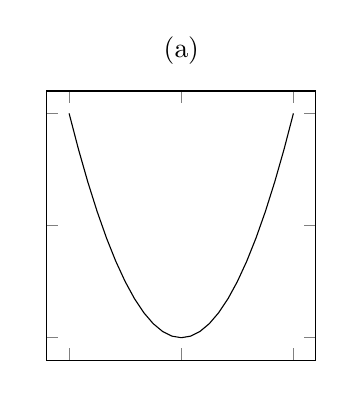
\begin{tikzpicture}
    \begin{axis}[
        width=5cm,
        height=5cm,
        title={(a)},
        % label style={font=\small},
        % xlabel={$x$},
        % ylabel={$f(x)$},
        yticklabels={,,},
        xticklabels={,,},
      ]
      \addplot[domain=-1:1] {x^2};
    \end{axis}
  \end{tikzpicture}%
  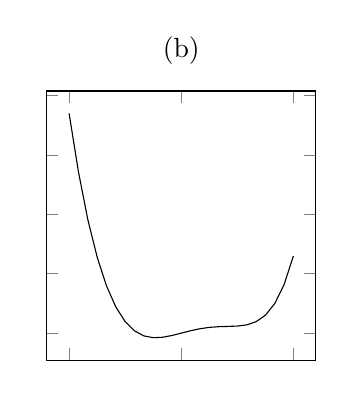
\begin{tikzpicture}
    \begin{axis}[
        width=5cm,
        height=5cm,
        title={(b)},
        % label style={font=\small},
        % xlabel={$x$},
        % ylabel={$f(x)$},
        yticklabels={,,},
        xticklabels={,,},
      ]
      \addplot[domain=-1:1] {x - 5*x^3 + 5*x^4 + 1.6*x^5};
    \end{axis}
  \end{tikzpicture}%
  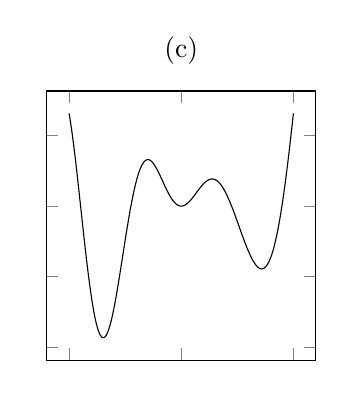
\begin{tikzpicture}
    \begin{axis}[
        width=5cm,
        height=5cm,
        title={(c)},
        % label style={font=\small},
        % xlabel={$x$},
        % ylabel={$f(x)$},
        yticklabels={,,},
        xticklabels={,,},
      ]
      \addplot[domain=-1:1, samples=1000] {sin(deg(7*x))*(x^4 - x^2 + x)};
    \end{axis}
  \end{tikzpicture}%
  \begin{tikzpicture}
    \begin{axis}[
        width=5cm,
        height=5cm,
        title={(d)},
        % label style={font=\small},
        % xlabel={$x$},
        % ylabel={$f(x)$},
        yticklabels={,,},
        xticklabels={,,},
      ]
      \addplot[solid, mark=none]
        table[x expr=\coordindex+1, y index=0] {plots/energy_landscape.csv};
    \end{axis}
  \end{tikzpicture}%
  \caption{Convex functions like the one shown in (a) can be minimized extremely
  efficiently even on high-dimensional domains. While the second example (b) is
  not convex anymore, it is smooth and has a unique minimum. Therefore local
  iterative methods will do an excellent job and converge quickly to the
  minimum. Function (c) is still smooth, but has several minima. Depending on
  where we position the starting point, iterative gradient methods might get
  stuck in one of the two local minima on the right and not find the global
  minimum on the left. The fourth function (d) is not even once differentiable
  and has numerous minima. We can only use heuristics and hope to get close to
  the true minimum.}
\label{fig:samplefuncs}
\end{figure}

The domain of our specific spin lattice optimization problem is a~$2 N_x N_y
N_z$-dimensional space.  Even for relatively small lattices optimization in such
a high-dimensional space is generically hard. Unfortunately, it appears
completely hopeless to compute the gradient or even Hessian of the
Hamiltonian~\eqref{hamiltonian} analytically. Moreover, it is hard to develop
intuition about how the energy landscape looks like, not only because we can
barely visualize anything in more than three dimensions. It appears certain,
however, that it will include a vast number of local minima with rough hills and
valleys. All of this is bad news for efficient iterative methods and we have to
fall back to heuristics. Our only option is to sample the search space
preferably in a smart and structured way and hope to capture the minimum within
reasonable computation time. This is precisely what Monte Carlo methods do. They
consist of a sampling strategy that involves some randomness. As was the case
for integration, this is horrifically inefficient. By now we understand why
Monte Carlo techniques should only be considered once everything else failed or
proved intractable.
%
%%%%%%%%%%%%%%%%%%%%%%%%%%%%%%%%%%%%%%%%%%%%%%%%%%%%%%%%%%%%%%%%%%%%%%%%%%%%%%%%
\section{The Metropolis algorithm}\label{sec:metropolis}
%%%%%%%%%%%%%%%%%%%%%%%%%%%%%%%%%%%%%%%%%%%%%%%%%%%%%%%%%%%%%%%%%%%%%%%%%%%%%%%%
%
For our use case we implemented \newterm{simulated annealing}. The name already
hints towards thermodynamic processes, which we identified to be a key
feature of our system, but were not yet able to bake it into our model. Clearly
any real material at finite temperature is not completely static, \ie{} stuck in
a fixed state~$\pi \in \Pi$, but it is constantly subject to thermal
fluctuations. Apparently our current objective, finding a unique global minimum
of the Hamiltonian for given parameters, is insufficient. Simulated annealing is
designed to mimic real world systems at finite temperature and will take care of
thermal fluctuations. That implies that we will not seek to find a single best
state~$\pi \in \Pi$ anymore, but consider the physical state to be a thermal
average of several configurations. For precisely these averages our discussion
of Monte Carlo integration will come in handy. To fully understand and
appreciate simulated annealing, we need some basic concepts from statistical
physics.

\subsection{Statistical physics in a nutshell}

In macroscopic complex many body systems such as gases or condensed matter at
finite temperature, we are often not interested in every single detail of that
system at a given moment in time.  For example, we do not want to know the
position and velocity as well as rotational and vibrational modes of each single
molecule in a piston. Sensible observables are typically some sort of
macroscopic averages like the volume, temperature or pressure of the gas. For a
solid we might be interested in its specific heat, conductivity or
susceptibility rather than the joint many body wavefunction of all electrons.
Statistical physics provides a sound and rigorous way to define those averages.

Instead of working with the complete microstates, in our case the elements
of~$\Pi$, directly, we only talk about the probability~$P_{T}(\pi)$ that the
system is in a certain state~$\pi \in \Pi$ at temperature~$T$. To this end we
imagine a large ensemble of exact replicas of the system and observe them all at
the same time figuratively counting how often each microstate occurs. Starting
from the assumption that in a closed system in equilibrium each microstate~$\pi$
is equally likely, we can derive the so called \newterm{canonical ensemble}. It
states that for a non-closed system in equilibrium at finite temperature~$T$,
\eg{} via contact to a large heat bath, the probability of state~$\pi$ is
%
\begin{equation}\label{boltzmann}
  P_{T}(\pi) = \frac{\exp \left(- \frac{H(\pi)}{k_B T}\right)}
  {\sum_{\pi \in \Pi} \exp \left(- \frac{H(\pi)}{k_B T}\right)}\:.
\end{equation}
%
This is also referred to as the \newterm{equilibrium Boltzmann distribution}
with~$k_B$ being the Boltzmann constant. For a finite configuration space these
are discrete probabilities that add up to one by construction. The normalizing
factor in~\eqref{boltzmann}
%
\begin{equation}
  Z := \sum_{\pi \in \Pi} \exp(-\beta H(\pi))
\end{equation}
%
is called \newterm{partition function}. Here we introduced the common
shortcut~$\beta := {(k_B T)}^{-1}$. In our case,~$\Pi$ consists of infinitely
many states and the summation in the partition function has to be replaced by an
integral
%
\begin{equation}
  Z := \int_{\Pi} \exp(-\beta H(\pi)) \sucd{\mu}_{\Pi}(\pi)\:,
\end{equation}
%
where the measure~$\mu_{\Pi}$ depends on the configuration space. In our case it
is a product measure of the standard measure on~$S^2$, but the mathematical
details are not important for the further treatment in this report. Note that we
will always consider the equilibrium Boltzmann distribution for a fixed
temperature~$T$ and somtimes drop the subscript~$T$ and simply denote it by~$P$.

The equilibrium Boltzmann distribution~\eqref{boltzmann} tells us that
configurations with lower energy are exponentially more likely than
configurations with higher energy. Furthermore, this effect is most pronounced
at low temperatures. If~$T$ is large, states with higher energy still occur with
a decent probability compared to the minimizing state. On the other hand, for~$T
\to 0$ basically only the state with minimal energy has a non-zero probability.
Both facts match our intuition. At high temperatures, thermal fluctuations are
large and the system can visit many different microstates. At zero temperature
we expect the system to settle in the ground state.

In a probabilistic description of states, the energy or magnetization of one
single specific configuration looses its significance. Instead we measure
expectations values of observables. For an observable~$\map{\cO}{\Pi}{\bR}$ we
compute the so called \newterm{thermal average}
%
\begin{equation}\label{thermavgsum}
  \avg{\cO} := \frac{1}{Z} \sum_{\pi \in \Pi} \cO(\pi) \exp(- \beta H(\pi))\:,
\end{equation}
%
hence we average over all states weighted by their probability at a given
temperature. For a continuous state space this becomes
%
\begin{equation}\label{thermavgint}
  \avg{\cO} := \frac{1}{Z} \int_{\Pi} \cO(\pi) \exp(- \beta H(\pi))
    \sucd{\mu}_{\Pi}(\pi)\:.
\end{equation}
%
In our case the observables we are primarily interested in are the
energy~$\avg{H}$ and the three components of the magnetization~$\avg{\M} =
\avg{\sum_{\r \in \Sigma} \S_{\r}}$.

One question immediately poses itself: How could be possibly compute the
high-dimensional integral in~\eqref{thermavgint} for our specific situation?
Even for finite configuration spaces the sum in~\eqref{thermavgsum} would
contain extraordinarily many terms. If each lattice site could only be in two
states, up or down, already on a small~$10^3$ lattice we would have to sum
up~$2^{1000} \approx 10^{300}$ configurations. This is far beyond the
possibilities of any machine imaginable today. The large dimensionality of the
problem renders it a good fit for Monte Carlo methods.
Indeed~\eqref{thermavgint} bears striking resemblance to~\eqref{probform}. The
standard measure on~$S^2$ can be derived from the Lebesgue measure~$\lambda^3$
on~$\bR^3$ and~\eqref{boltzmann} is the probability density function~$p$
on~$\Pi$. It assigns almost no weight to configurations with high energy. As a
consequence they will not contribute much to the integral and the thermal
average calls for importance sampling
%
\begin{equation}\label{thermavgapprox}
  \avg{\cO} \approx \frac{1}{N} \sum_{i = 1}^N \cO(\pi_i)\:,
\end{equation}
%
where~$\pi_i$ are independent samples drawn from the Boltzmann
distribution~$P_T$. Finally we see how Monte Carlo integration enters the
picture.

\subsection{Generating random configurations}\label{subsec:random}

The challenge is to generate independent random samples following the Boltzmann
distribution~\eqref{boltzmann}. Generating a uniformly random sample is
relatively easy, although there is one major pitfall one has to look out for.
The strategy is of course the pick a uniformly random spin at each vertex of the
grid. Some implementations claim to generate uniformly random elements of~$S^2$
in the following way. They generate three random numbers~$x,y,z \sim
\cU_{[-1,1]}$ and then normalize the resulting vector~$(x,y,z) / \sqrt{x^2 + y^2
+ z^2}$. While~$(x,y,z)$ in this case is uniformly distributed on the
cube~$[-1,1]^3$, by simply projecting all points onto the sphere~$S^2 \subset
[-1,1]^2$, the points that were originally generated outside the sphere,
\ie{}~$[-1,1]^3 \setminus B^3$, are unevenly distributed. Here the unit
ball~$B^3$ is the interior of~$S^2$. The corners of the cube host more points
than the areas where the sphere actually touches the boundary of the cube and
thus we expect more points in a small neighborhood around~$3^{-1/2} (1,1,1)$
than around~$(0,0,1)$.

There are several ways to mitigate this effect. One is to discard all
points~$(x,y,z)$ with length greater than one and redraw new points in the cube
until they fall inside the sphere. We do not recommend this method, because of
its inefficiency. In three dimensions we have~$\lambda^3([-1,1]^3) =
8$,~$\lambda^3(B^3) = 4 \pi / 3$ and thus
%
\begin{equation}
  \frac{\lambda^3([-1,1]^3 \setminus B^3)}{\lambda^3([-1,1]^3)} \approx 0.476\:,
\end{equation}
%
\ie{} one would have to discard almost every second vector. The ratio becomes
ever larger in higher dimensions. A slightly better way is make use of the fact
that~$S^2$ is a two-dimensional manifold, thus can be parameterized by only two
real numbers. One can independently draw~$x,y \sim \cU_{[-1,1]}$, discard and
redraw them if~$x^2 + y^2 > 1$ and otherwise return
%
\begin{equation}
  \begin{pmatrix}
    2 x \sqrt{1 - x^2 - y^2} \\
    2 y \sqrt{1 - x^2 - y^2} \\
    1 - 2 (x^2 + y^2)
  \end{pmatrix} \:,
\end{equation}
%
which results in a uniform distribution on the sphere. This is a slight
improvement, because we only discard the fraction
%
\begin{equation}
  \frac{\lambda^2([-1,1]^2 \setminus B^2)}{\lambda^2([-1,1]^2)} \approx 0.215\:,
\end{equation}
%
but still not optimal. Interestingly, the original
method~$(x,y,z)/\norm{(x,y,z)}$ works if we draw~$x,y,z$ from a normal
distribution with mean zero. The downside of this approach is that the
generation of normally distributed random numbers is slightly slower than
uniformly distributed ones.

Finally, let us describe the method we used in our implementation. In the final
implementation we prefer the redundant representation as three-dimensional
vectors, because it simplifies the computation of dot and cross products as well
as projections onto coordinate planes. Nevertheless for the generation of
uniformly random spins on~$S^2$ it is advantageous to work in spherical
coordinates~$(\phi, \theta) \in [0,2\pi) \times [0,\pi)$. The next pitfall is
already waiting for us. Uniformly chosen~$\phi$ and~$\theta$ will also not
result in a uniform distribution on~$S^2$, because the density of points would
be larger near the north and south pole, \ie{} for~$\theta$ near~$0$ and~$\pi$
than near the equator~$\theta=\pi/2$. One could also anticipate this from the
fact that the coordinate transformation from spherical to Euclidean coordinates
is not isometric. We have to take into account the Jacobian
factor~$\sin(\theta)$ in the transformation. The correct procedure is hence the
following:
%
\begin{enumerate}
  \item Draw~$z \sim \cU_{[-1,1]}$ and~$\phi \sim \cU_{[0,2\pi)}$.
  \item Compute~$r_{xy} = \sqrt{1 - z^2}$.
  \item The vector~$(r_{xy} \cos(\phi), r_{xy} \sin(\phi), z)$ is a sample
    from~$\cU_{S^2}$.
\end{enumerate}
%
Here we make use of the fact that the~$z$ component, \ie{}~$\cos(\theta)$, of
uniformly distributed points on~$S^2$ is uniformly distributed on~$[-1,1]$. The
azimuthal angle~$\phi$ is also uniformly distributed on~$[0,2\pi)$. The~$x$
and~$y$ components are then computed such that the resulting vector has unit
length. Note that for all intervals above it does not matter whether we include
the end points or not, because they constitute a null set with respect to the
Lebesgue measure. In our benchmarks the latter method was almost a factor two
faster than all other options.

By now we have still only clarified how to generate a uniformly random
configuration~$\pi \sim \cU_{\Pi}$. The whole purpose of the simulated annealing
algorithm is to generate independent configurations from the Boltzmann
distribution which we need to estimate the integral~\eqref{thermavgint}.
Equation~\eqref{thermavgint} makes it very clear that we have to drop the notion
of finding a minimizing state of the energy. The observable energy~$\avg{H}$ is
a weighted average over all possible states. At finite temperature we can
therefore impossibly speak of a single best one. Consequently the optimization
aspect is an implicit feature of simulated annealing in the following sense.
Because simulated annealing helps us to generate configurations drawn randomly
from the Boltzmann distribution, most of its sample configurations will have
rather low energy depending on the temperature. Hence it implicitly drives the
system into states of low energy. Particularly as~$T \to 0$, it will inevitably
end up in low energy states. As it is just a heuristic, we have no guarantee
whether it will actually find a global minimum at~$T=0$, but that would be the
desired outcome. Now let us finally explore how simulated annealing manages to
sample the Boltzmann distribution.

\subsection{Markov chains}

The crucial idea is to not create each random sample completely from scratch,
but to slowly work towards more likely configurations. If we simply pick a
uniform random configuration, we can only evaluate its energy once it has been
generated. It would take a huge number of samples to figure out which energies
are relatively high and therefore unimportant, or relatively low and therefore
contribute a lot. Even if we knew the energy range up front, we could not
generate configurations in a certain energy range from scratch, but only decide
after we have generated it.

The cure for this problem are so called \newterm{Markov chains}. In a Markov
chain we start at any configuration~$\pi_0$ and modify that configuration to
transition to the next one~$\pi_1$. Then we continue from there, which yields
the following picture
%
\begin{equation}
  \xymatrix{\pi_0 \ar[r]^{\phi} &\pi_1 \ar[r]^{\phi} &\pi_2 \ar[r]^{\phi}
  &\;\cdots}
\end{equation}

The transition procedure, which we denoted by~$\phi$, has to fulfill two
requirements. At some point we want configuration~$\pi$ to occur in the chain
with probability~$P_T(\pi)$, \ie{} it has to actually sample the Boltzmann
distribution. The second requirement stems from the fact that for Monte Carlo
integration to work we need independent samples. Since~$\pi_{i}$
now clearly depends on all~$\pi_j$ with~$j < i$, we have to make sure
that~$\phi$ modifies each state enough to render the next one practically
independent of its predecessor. We can characterize~$\phi$ by the probability
with which it transforms state~$\pi$ into state~$\pi'$. For each pair of
states~$\pi, \pi' \in \Pi$ we denote the transition probability by~$\T(\pi \to
\pi')$. Proper transition probabilities have to fulfil
%
\begin{equation}\label{probprop}
  \sum_{\pi' \in \Pi} \T(\pi' \to \pi) = 1 \qqtxtqq{or}
  \int_{\Pi} \T(\pi' \to \pi) \sucd{\mu}_{\Pi}(\pi') = 1
\end{equation}
%
meaning that starting from~$\pi$ the system has to go to \emph{some} other state
in the configuration space.

\subsubsection{State transitions of a spin lattice}

For illustration purposes let us explain what the transition process~$\phi$ will
look like in our specific example. The simplest way to modify a state~$\pi \in
\Pi$ is to pick one of the spins~$\S_{\r} \in S^2$ and change it. Since we have
no indicators as to which spin we should change and how to modify it to bring
the new state close to a sample from the Boltzmann distribution, we follow the
Monte Carlo scheme and select the position~$\r \in \Sigma$ as well as the new
spin~$\S'_{\r}\in S^2$ uniformly at random, respectively. Obviously flipping one
spin out of many does not yet result in an independent state, in fact the
correlation between the two configurations would be almost one. Thus~$\phi$ has
to consist of a little more than just changing one spin, which we will
henceforth call an \newterm{update}. Instead, we change many spins and we change
them often. Successively updating~$|\Sigma| = N_x N_y N_z$ random vertices is
called one \newterm{lattice sweep} or just \newterm{sweep}. The
transition~$\phi$ from one configuration to the next will consist of~$\Nsweep
\in \bN$ many lattice sweeps. Thus, between two successive configuration each
lattice site has been updated~$\Nsweep$ many times on average, see
\figref{fig:update}. The exact number~$\Nsweep$ has to be determined by careful
analysis such that~$\pi_{i+1}$ is independent of~$\pi_i$. Apparently, if we
simply keep updating spins in that fashion, each transition will have the same
probability and we only generate uniformly random samples of~$\Pi$ instead of
drawing from the Boltzmann distribution. By carefully selecting which updates
actually are allowed to happen and which we reject without any changes to the
current state, we can tune the transition probabilities to our liking. Before we
go into that, however, we have to determine what the transition probabilities
have to be.

\begin{figure}
  \centering
  \begin{tikzpicture}
    \draw[thick] (0,0) -- +(0.5,0) node[pos=0, left] {$\pi_i$};
    \draw[->,>=latex, thick] (13.3,0) -- +(0.5,0) node[pos=1, right] {$\pi_{i+1}$};
    \begin{scope}[xshift=6cm]
      \config{}
    \end{scope}
  \end{tikzpicture}
  \caption{To render state~$\pi_{i+1}$ independent of state~$\pi$, we
  perform~$\Nsweep$ sweeps, each consisting of~$|\Sigma|$ individual spin
  random changes.}
\label{fig:update}
\end{figure}

\subsubsection{Transition probabilities}

Let~$P_i(\pi)$ be the probability that at the~$i$-th step of
the chain we are in state~$\pi$. This probability can be computed recursively.
What is the probability that at step~$i+1$ we are in state~$\pi$? There are
basically two ways we could end up there. Either we were in a different
state~$\pi'$ at the~$i$-th step and hit the transition probability~$\T(\pi' \to
\pi)$, or we have already been in~$\pi$ and stayed there, which happens with
probability~$\T(\pi \to \pi)$. Those can be combined into
%
\begin{equation}\label{master}
  P_{i+1}(\pi) = \sum_{\pi' \in \Pi} P_i(\pi') \T(\pi' \to \pi) \qqtxtqq{or}
  P_{i+1}(\pi) = \int_{\Pi} P_i(\pi') \T(\pi' \to \pi) \sucd{\mu}_{\Pi}(\pi')\:.
\end{equation}
%
Let us refactor this expression, using only the summation notation, because it
is simpler and can trivially be transformed into the continuous version.
With~\eqref{probprop}, we find
%
\begin{align}\label{masterlong}
  P_{i+1}(\pi) &= \sum_{\pi' \in \Pi} P_i(\pi') \T(\pi' \to \pi) +
    P_i(\pi) (1 - \sum_{\pi' \in \Pi} \T(\pi \to \pi')) \\
  &= P_i(\pi) + \sum_{\pi' \in \Pi}
    (P_i(\pi') \T(\pi' \to \pi) - P_i(\pi) \T(\pi \to \pi'))\:.
\end{align}
%
In this form we can interpret the first term of the sum as all the ways we can
enter state~$\pi$ at step~$i+1$ and the second term as all the ways we can leave
state~$\pi$ in step~$i+1$. This form will prove helpful in a moment.

Now we aim at tuning the transition probabilities such that~$\lim_{i \to \infty}
P_i = P$, \ie{} the probabilities in~\eqref{master} converge to a stationary
distribution that agrees with the Boltzmann distribution~\eqref{boltzmann}. In a
stationary distribution, the probability of entering a certain state has to be
equal to the probability of leaving that state. If we entered a state more often
than we left it or vice versa, the distribution would clearly not be stationary.
Mathematically this signifies that we can tune the transition probabilities such
that the terms of the sum in~\eqref{masterlong} cancel each other out. In the
limit~$i \to \infty$, where~$P_i(\pi) = P(\pi)$ for all states~$\pi \in \Pi$, we
find
%
\begin{equation}\label{detbal}
  P(\pi') \T(\pi' \to \pi) = P(\pi) \T(\pi \to \pi')\:.
\end{equation}
%
This condition is called \newterm{detailed balance} and is a key feature of
Markov chains. We can interpret it as reversability of the transition
process~$\phi$. Going from~$\pi$ to~$\pi'$ is equally likely as the other way
round.

\subsubsection{The Metropolis algorithm}

The ratio of the transition probabilities reveal another interesting
aspect
%
\begin{equation}
  \frac{\T(\pi \to \pi')}{\T(\pi' \to \pi)} = \frac{P(\pi')}{P(\pi)} =
  e^{-\beta (H(\pi') - H(\pi))} =: e^{-\beta \Delta H}\:.
\end{equation}
%
Thus the transition probabilities depend only on the energy difference of the
two states in question. In particular it does not remember previous states. At
each step we can decide  the transition probability purely from the current and
the proposed successor configuration. This property is our main guidance in
engineering the transition probabilities. One rather obvious choice is given by
%
\begin{equation}
  \T(\pi \to \pi') = \min(1, e^{-\beta (H(\pi') - H(\pi))})\:.
\end{equation}
%
Those are the so called \newterm{Metropolis} (or \newterm{Metropolis-Hastings})
transition probabilities. The whole Markov chain Monte Carlo integration for
thermodynamic systems like ours using the Metropolis transition probabilities is
simply called \newterm{Metropolis algorithm} or \newterm{Metropolis-Hastings
algorithm}. There are also other valid choices for the transition probabilities,
for example the so called \newterm{Heatbath algorithm}, but we will only discuss
and implement the Metropolis algorithm.

Now that we know the transition probabilities we can bake them into our state
transition procedure~$\phi$. Recall that~$\phi$ consists of~$\Nsweep$ lattice
sweeps, each of which performs~$|\Sigma|$ random updates of single spins. Each
time we have selected a spin~$\S_{\r}$ from the current configuration~$\pi$ for
an update, we will first generate its potential replacement~$\S'_{\r} \sim
\cU_{S^2}$, which would lead to state~$\pi'$. But now we only actually perform
the update, if
%
\begin{equation}
  T(\pi \to \pi') > \cU_{[0,1)}\:.
\end{equation}
%
In this way we abide to the desired transition probabilities in each update,
thus in each sweep and eventually also in each complete transition~$\phi$.

For completeness, let us mention that the second key requirements for Markov
chains to work properly besides detailed balance is \newterm{ergodicity}.
Ergodicity says that each state must be reachable from every other state in a
finite number of steps. We are not going to elaborate on the theoretical
importance of this property. We point out, however, that ergodicity is clearly
fulfilled in our specific model, because we have to change a maximum of~$N_x N_y
N_z$ spins and each possible spin flip has non-zero probability.

\subsubsection{Thermalization and the start configuration}

Theoretically a Markov chain can go on forever, traversing through different
states, each time choosing the successor configuration at random according to
the transition probabilities. Given detailed balance and ergodicity, after
sufficiently many steps, we have converged to a stationary distribution and each
new state can be considered an independent sample from the Boltzmann
distribution. Those initial steps before the distribution becomes stationary are
called \newterm{thermalization}. The close ties to thermodynamics are obvious,
where a system can only be treated statistically, if it is in thermal
equilibrium, \ie{} after it has thermalized. Hence, before we can actually use
the states~$\pi_i$ as independent samples of the Boltzmann distribution to
estimate thermal averages via~\eqref{thermavgapprox}, we have to
perform~$\Ntherm$ lattice sweeps to equilibrate the system. Henceforth the
time~$t$ is measured by the number of lattice sweeps we have performed. While
detailed balance and ergodicity guarantee that there is some finite~$\Ntherm \in
\bN$, the precise value depends on a number of factors.

First of all it depends on the start configuration. In lattice models like ours
the two most commonly used options are a \newterm{hot start} or a \newterm{cold
start}. In a hot start we initialize the first state uniformly at random~$\pi_0
\sim \cU_{\Pi}$.  Practically that means that we initialize each spin~$\S_{\r}$
for~$\r \in \Sigma$ independently uniformly at random~$\S_{\r} \sim \cU_{S^2}$
as discussed in subsection~\ref{subsec:random}. It is called hot start, because
in the limit~$T\to \infty$ the Boltzmann distribution becomes a uniform
distribution and each state is equally likely. Hence at infinite temperature a
hot start already follows the Boltzmann distribution and the system is in
thermal equilibrium from the very beginning. In a cold start all spins are
chosen the same into some direction, possibly parallel to the external magnetic
field, which corresponds to a global minimum of the Hamiltonian  including only
direct exchange and the Zeeman energy at zero temperature.

Secondly, the thermalization time varies with temperature. We have already seen
that at high temperatures almost all transitions have a decent probability and
we can explore many states in a short time, guiding the system into equilibrium
faster. At very low temperatures the Boltzmann distribution is highly localized,
peaked at low energy states and we will have to reject many proposed successors
before we discover the probable configurations. Generally this yields a long
thermalization time for low temperatures.

Thirdly, the system size plays a crucial role. The equilibration time
unsurprisingly grows directly with the system size. This can be understood
easily simply from the fact that in a large system it takes longer for all parts
of it to communicate with each other and find a joint equilibrium state. We will
discuss in the next section, how one can detect when the system is fully
equilibrated. From here on we will consider~$\pi_0$ to be the initial
configuration and~$\pi_1$ to be the first configuration after thermalization,
\ie{} the first one that can actually be used to compute thermal averages.
Afterwards all following configurations are separated by~$\Nsweep$ sweeps.

\subsection{Summary and pseudocode}

The ultimate goal of the Metropolis algorithm is to estimate observables such as
the energy or the magnetization at fixed temperature~$T$ and external field~$B$.
Therefore it has to output the collection of desired observables, which we
denote generically by~$\cO$, for~$N$ independent samples of the Boltzmann
distribution. Let us now put all the pieces together and lay out a pseudo code
for the Metropolis algorithm at fixed temperature~$T$ and external field~$B$ in
algorithm~\ref{alg:metropolis}. The full metropolis algorithm can be depicted
schematically as

\begin{equation}
  \xymatrix{%
    \text{initialize} \ar[d]
      &\text{save } \cO(\pi_1)
      &\text{save } \cO(\pi_2)
      && \text{save } \cO(\pi_N) \\
    \pi_0 \ar[r]^{\Ntherm}_{\text{sweeps}}
    & \pi_1 \ar[r]^{\Nsweep}_{\text{sweeps}} \ar[u]
    & \pi_2 \ar[r]^{\Nsweep}_{\text{sweeps}} \ar[u]
    & \cdots \ar[r]^{\Nsweep}_{\text{sweeps}}
    & \pi_N \:. \ar[u]
  }
\end{equation}

\begin{algorithm}
  \caption{Metropolis algorithm}\label{alg:metropolis}
  \begin{algorithmic}[1]
    \Require{Initialize the spin lattice, \eg{} with a hot start~$\pi_0 \sim
    \cU_{\Pi}$.}
    \Statex
    \Procedure{metropolis}{$\pi_0$, $T$, $B$} \Comment{$T, B$ are fixed}
      \For{$i$ from~$1$ to~$\Ntherm$} \Comment{thermalization}
        \State \textsc{sweep}($\pi_0$)
      \EndFor
      \State set $\pi_1 := \pi_0$
      \State save~$\cO(\pi_1)$
      \For{$i$ from~$1$ to~$N-1$}
        \State set $\pi_{i+1} :=$ \textsc{next\_config}($\pi_i$)
        \State save~$\cO(\pi_{i+1})$
      \EndFor
    \EndProcedure
    \Statex
    \Function{next\_config}{$\pi$}
      \For{$j$ from~$1$ to~$\Nsweep$}
        \State \textsc{sweep}($\pi$)
      \EndFor
      \State \Return{$\pi$}
    \EndFunction
    \Statex
    \Procedure{sweep}{$\pi$} \Comment{\textsc{sweep} modifies~$\pi$}
      \For{$i$ from~$1$ to $N_x N_y N_z$}
        \State draw $\r \sim \cU_{\Sigma}$
        \State draw $\S' \sim \cU_{S^2}$
        \If{$\min\bigl(1, \exp(- \beta \Delta H)\bigr) >
          \mathrm{rand}(0,1)$}
            \State replace~$\S_{\r} \in \pi$ by~$\S'_{\r}$
        \EndIf
      \EndFor
    \EndProcedure
  \end{algorithmic}
\end{algorithm}

%
%%%%%%%%%%%%%%%%%%%%%%%%%%%%%%%%%%%%%%%%%%%%%%%%%%%%%%%%%%%%%%%%%%%%%%%%%%%%%%%%
\section{Analysis and statistics}\label{sec:analysis}
%%%%%%%%%%%%%%%%%%%%%%%%%%%%%%%%%%%%%%%%%%%%%%%%%%%%%%%%%%%%%%%%%%%%%%%%%%%%%%%%
%
In the previous sections we discussed the Metropolis algorithm and provided a
pseudocode which should make it fairly easy to implement. However, we issued
quite a few warnings without giving specific instructions on how to stay on the
safe side of things. How should one choose the thermalization time~$\Ntherm$ and
how do we know whether the system is in equilibrium? How large does~$\Nsweep$
have to be such that consecutive configurations of the Markov chain can be
considered independent? In this section we try to answer this question or at
least provide some practical guidelines.

\subsection{Thermalization}

Equilibration is a sensitive and often underestimated topic. It is by far not
sufficient to let ``a few sweeps'' go by after a hot start, even at high
temperatures. In the literature one can find guidelines that suggest that the
thermalization time should be at least~$15-20$\% of the total runtime. The total
runtime, as always measured in Monte Carlo time, \ie{} the number of lattice
sweeps, is given by~$\Ntherm + N\cdot \Nsweep$. Such estimates, while helpful to
get an idea of the order of magnitude, often lure scientists into blindly
allocating~$20$\% of the overall runtime for equilibration and feel on the safe
side. This is plain wrong and indefensible. Despite all the factors that go into
the thermalization time, the number of sweeps in between configurations and the
overall number of configurations one chooses to compute are not among them. How
could one expect the thermalization time to decrease only because we stop the
Markov chain after just a few configurations? Those are just the most obvious
flaws in absolute recommendations. Besides the system size, the temperature and
the start configuration the equilibration time also differs for various
observables and of course for different systems and models. We cannot expect to
find a solution without closely analyzing the specific final implementation of
the model at hand.

That being said, even then there is no~$100$\% foolproof recipe to
determine~$\Ntherm$ in a fully satisfying fashion. The most common approach is
to simply look at the observables one is interested in. After the implementation
is finished and before we actually start to record states of the Markov chain,
we write out \emph{all} observables we are interested in after every single
sweep beginning right with the initialing state. If one is interested in the
energy and the magnetization of the system, one would plot the energy and all
three components of the magnetization over Monte Carlo time~$t$, \ie{} over the
number of sweeps. In \figref{fig:thermalization} we see that all observables
level out over time and then merely fluctuate around a constant value. This
happens much later for the magnetization than for the energy. Thus it is vital
to look at such plots for all observables one ever plans to look at. The point
from which onwards all observables are basically constant is the minimal
equilibration time for this specific system with those specific parameters.

\todo{figure of thermalization}

Keep in mind that in principle one has to repeat this analysis whenever one
changes the temperature, the system size, the magnetic field or any other
parameters of the model. Since hot start conditions are chosen at random, even
the exact same simulation with a different start configuration could have a
longer or shorter thermalization time. Therefore a generous additional cushion
is mandatory. Analyzing and determining~$\Ntherm$ for the whole range of
parameters one intends to simulate is the very first step after the Metropolis
algorithm has been implemented and tested exhaustively for correctness.

\subsection{Autocorrelation}

Another pitfall we have emphasized several times already is the necessity of
\emph{independent} samples for Monte Carlo integration to work properly. Our
samples are the states of a Markov chain with the generic characteristic that
each state is generated by modifying its predecessor. By definition the
resulting samples are not independent. However, by separating subsequent
configurations by sufficiently many Monte Carlo steps we can bring down their
correlation until they can be considered independent for all practical purposes.
We will now quantify how~$\Nsweep$ has to be chosen to guarantee such
independence.  Again it does not seem too harmful to simply let a ``good amount
of'' sweeps go by in between consecutive configurations of the Markov chain, but
there is actually analytic evidence that one has to take correlations seriously.

\newterm{Autocorrelation} is \emph{the} central tool to quantify correlations of
individual states within a time series. Given an observable~$\cO$ at Monte Carlo
times~$\numlist{1}{N}$, where we start counting once the system has thermalized,
the autocorrelation function can be estimated
%
\begin{equation}
  R_{\cO}(t) := \frac{1}{\sigma^2 (N-t} \sum_{i = t}^{N}
    (\cO(i) - m) (\cO(i+t) - m)\:,
\end{equation}
%
where~$\sigma^2$ is the variance and~$m$ the mean of the energy. Note that it
only makes sense to talk about the mean and variance once we draw from a
stationary distribution, \ie{} after the system has thermalized.  Since we do
not have access to the true mean and variance of the entire system in thermal
equilibrium at a fixed temperature we have to estimate those quantities too. We
use the standard sample mean and sample variance of~$\numlist{\cO(1)}{\cO(N)}$
%
\begin{equation}\label{autocorr}
  m = \frac{1}{N} \sum_{i=1}^N \cO(i) \qqtxtqq{and}
  \sigma^2 = \frac{1}{M-1} \sum_{i=1}^N (\cO(i) - m)^2
\end{equation}
%
which makes~$R_{cO}$ a biased estimate. A few remarks are in order. The
autocorrelation can be understood as the covariance of the sequence with a
shifted version of it. Since we want to measure the correlation of states at
different time in the same chain this is entirely plausible. Like the
covariance, the autocorrelation can become negative which is interpreted in the
same way. Negative autocorrelation at time~$t$ means that large negative values
of~$\cO$ at a certain time correlate with large positive values~$t$ steps later
in the chain. The variance in the denominator normalizes the autocorrelation to
lie in~$[-1,1]$. One major issue with the estimator~$R_{\cO}$ is due to the fact
that we are dealing with a finite sequence of measurements. The sum
in~\eqref{autocorr} runs over fewer and fewer terms the larger~$t$ becomes,
because the possible overlap between the original and the time-shifted sequence
decreases. However, we need a certain terms in the sum to average out random
fluctuations and keep the variance of our estimate for the autocorrelation small
enough. Therefore it only makes sense to look at~$R_{\cO}$ for~$t \ll N$.

The autocorrelation function in Markov chain Monte Carlo simulations generically
decays like~$\exp(-t/\tau)$, where~$\tau$ is called \newterm{autocorrelation
time}.

\todo{continue with autocorrelation analysis, show that autocorrelation alters
error estimates, integrated autocorrelation time and plots}

\subsection{Errors}


\todo{what happened to simulated annealing? should i completely remove it from
the whole thing? if not, where do I add it? I could make a section in between
metropolis and analysis briefly explain it and write pseudocode wrapping the
metropolis function from above}

\subsection{General remarks}

\todo{looking at acceptance rates can give valueable insights}
